% This is LLNCS.DEM the demonstration file of
% the LaTeX macro package from Springer-Verlag
% for Lecture Notes in Computer Science,
% version 2.4 for LaTeX2e as of 16. April 2010
%
\documentclass{llncs}
%
\usepackage{makeidx}  % allows for indexgeneration
\usepackage{color} %vrivas, 15-Jan-2016
\usepackage{hyperref} %vrivas, 21-Jan-2016, for \url
\usepackage{graphicx} %vrivas, 27-Jan-2016, for images
\usepackage{listings}%vrivas, 27-Jan-2016, for code
%c
\begin{document}
%
\frontmatter          % for the preliminaries
%
\pagestyle{headings}  % switches on printing of running heads
\addtocmark{Web browser-based time-series forecasting} % additional mark in the TOC

%
\mainmatter              % start of the contributions
%
\title{Web browser-based forecasting of economic time-series}
%
\titlerunning{Web browser-based forecasting}  % abbreviated title (for running head)
%                                     also used for the TOC unless
%                                     \toctitle is used
%
\author{
V.M. Rivas\inst{1,3} \and E. Parras-Guti\'{e}rrez\inst{1}
\and JJ Merelo\inst{2,3}  \and M.G. Arenas\inst{2,3}
\and P. Garc\'{\i}a-Fern\'{a}ndez\inst{2,3}
}
%
\authorrunning{V. M. Rivas et al.} % abbreviated author list (for running head)
%
%%%% list of authors for the TOC (use if author list has to be modified)
\tocauthor{V M. Rivas}
%
%\institute{Depto. de Informatica, Univ. de Jaen, SPAIN,\\
\institute{Univ. of Jaen, Dept of Computer Sciences,\\
Campus Las Lagunillas s/n, 23071, Ja\'{e}n, SPAIN\\
\email{vrivas@ujaen.es}, 
\texttt{http://vrivas.es}
\and
Depto. de Arquitectura y Tecnolog\'{\i}as de las Computadoras\\
Depto. de Electr\'{o}nica y Tecnolog\'{\i}as de las Computadoras\\
Univ. de Granada, SPAIN
Univ. of Granada, Dept. of Computers, Architecture and Technology,\\
C/ Periodista Daniel Saucedo s/n, 18071, Granada, SPAIN
\and
GeNeura Team \\ \texttt{http://geneura.wordpress.com}
}

\maketitle              % typeset the title of the contribution
\begin{abstract}
Using the browser for running forecasting algorithms is a challenge,
since language support and performance varies across implementations
of the JavaScript virtual machine and vendor. However, using them will
provide a boost in the number of platforms available to
scientists. % A bit of motivation for the paper
% Papers need to have: motivation, objective. And the first sentences
% in the paragraph will have to go in that direction.
That is why  in this paper we present the implementation of a time series
forecasting algorithm, {\em jsEvRBF} that uses genetic algorithm and neural nets
in a way that can be run in must modern web browsers. {\em jsEvRBF} is
written in JavaScript, so that it can
be easily delivered to and executed by any device containing a
web-browser just accessing an URL. The experiments show the results
yielded by the algorithm over a  data set related to currencies
exchange. % the results are what? Good? Better? Worse?
Best results achieved  can be effectively compared against
previous results in literature, though robustness of the new algorithm
has to be improved. % What was your objective? Just running it?
                    % Running it with a decent performance? - JJ










\keywords{Time-series forecasting, evolutionary computation, radial basis function neural networks, Web-based programming, volunteer computation}
\end{abstract}
%
\section{Introduction}
% Web-based computing
%Web browsers stopped to be just simple HTML renders at the moment they allowed the executions of third-part programs included in the pages they downloaded. This way, browsers turned into wider frameworks in which multi-platform applications could be run. 
%Flash??? reference??? and Java applets the??? are probably the best known techniques to do this, even for non-experts users. But, in fact, 
Nowadays, most programs executed by browsers are written in a language called JavaScript, developed in an attempt to do the Web more dynamic \cite{Rauschmayer04}. 
Current everyday, massively-used web pages and applications (including those related to social networks) exist thanks to this language.
Its use has turned browsers into wider frameworks in which multi-platform applications can be run.
%The web, as we currently use it, would not be the same without the capability that JavaScript gives to the browser to make calculus, interact with the user, or dynamically retrieve data from servers without reloading the whole page, as it's done with AJAX Reference???. 
%Throughout the 1990s, the proprietary web browser Netscape Navigator had been created and was dominant, and in 1995, Brendan Eich was hired by Netscape company to design and implement a new language. At the same time, Netscape collaborated with Sun company to include in Navigator Java, its more static programming language, so it was questioned the needed of two programming languages: Java and a scripting language. Finally, they decided that the new scripting language had to make more accessible to non-Java programmers and web designers the support for Java applets \cite{Champeon08}. In May 1995, Eich designed a prototype in 10 days and was named first \emph{Mocha}, coined by the founder of Netscape Marc Andreessen, then \emph{LiveScript} and finally, in December 1995, \emph{JavaScript} \cite{Eich2010}, not because of the Java programming language, but to support Sun Microsystems.
JavaScript was standardized in 1997 by the European Computer Manufacturer's Association, or ECMA. According to the ECMA-262 standard, its real name is \emph{ECMAScript}, but everyone calls the language \emph{JavaScript} \cite{Flanagan06}.

% Restricciones de JavaScript
JavaScript can be described as a general-purpose, object-based, event-driven language.
% that can be used to write programs for both the client and the server REFERENCE-NODE???. T�
Adding JavaScript programs to web pages is simple: the code is inserted in the HTML code in plain text; then, it is downloaded by the browser that, finally,  interprets and executes it.
%Thus, although web browsers allow the users to change the preferences in order to disable the execution of any JavaScript code, this is rarely done in these days. Even more, most standard web users are not aware of the existence of this language, not realizing their browsers are working as programming environments in which code is analyzed, translated into a low-level language and executed. Consequently, and 
%For safety reasons, programs written in JavaScript are executed by browsers using a sandbox model. This model imposes a series of restriction that could be summarized as: the JavaScript program inserted in a given web page cannot access any other resources than the ones contained in that web page. JavaScript programs are allowed to the client's file system to store little pieces of text (called cookies), and also when the user has to select a file to be sent across the net.
Due to the abilities of JavaScript, in this work we propose the use of web browsers as agents able to download a web page containing a set of data, execute an evolutionary algorithm that evolves neural nets, and apply this neural nets to forecast an economic time-series. Using this approach, any device  able to execute a web browser (from computers to smart TVs) can be potentially used to run any algorithm.

% Genetic Algorithms and RBFNN
Both the problem being considered in this paper and the algorithm used to solve it were introduced in \cite{Rivas04}. On the one hand, the problem consists on forecasting the values of the
exchange rates between two currencies, for a four years period (data is weekly averaged). On the other hand, the algorithm (described in section \ref{sec:algorithm}) is a reduced version of {\em EvRBF}\cite{Rivas04}, an evolutionary algorithm that makes Radial Basis Function Neural Networks (RBFNN) to evolve.

RBFNN are well-known feed-forward neural nets with just one hidden and one output layers %\cite{Broomhead88}. They have been successfully used to solve classification, function approximation, and, as in this work, time-series forecasting 
\cite{Broomhead88,Keogh03,Whitehead} problems.
%The neurons in the output layer (only one neuron in this work) compute a weighted sum using outputs provided by hidden neurons, multiplied by some weights previously established, and adding a bias. The neurons in the hidden layer receive the input samples concerning the problem being resolved, and apply an activation function that  is a Radial Basis Function, i.e., a function returning a value that depends on the distance from the input values to a pre-established center of the function. The shape of this function is modified by means of a radius or width: the narrower this width, the higher the number of inputs that will not activate the neuron. Usually, Gaussian function is selected as the activation function, but many others can also be used.
Configuring an RBFNN in order to solve a task consists on: a) choosing the activation function for hidden neurons, b) choosing the number of hidden neurons, c) setting the parameters required by the activation functions (center and radius of the RBF), and d) setting the values for weights and bias. This last step can be easily computed once the rest of components have been established using the Least Mean Square method. {\em EvRBF} algorithm was designed to automatically search for the best configuration of an RBFNN that solves the problem being tackled, except for the activation function to be used that is always a Gaussian function.

% Time-series prediction

%Time-series can be considered as a special kind of function approximation where future values of the series are expressed as a function of past ones.
%There exist many methods in literature developed to forecast time-series references, being ARIMA \cite{BoxJenk} probably the most widely used.

In the herein, the implementation of {\em EvRBF} for web browsers (called {\em jsEvRBF}) has been compared to its original implementation as well as to the methods by \cite{Sheta2001}, the one introducing the data set tackled in this paper. Next sections describe: the algorithm (section \ref{sec:algorithm}); the problem to which the algorithm has been applied, as well as the experiments carried out  and the results yielded (section \ref{sec:experiments}), and conlusions and future lines (section \ref{sec:conclusions}).


\section{The {\em jsEvRBF} algorithm}
\label{sec:algorithm}
% The {\em EvRBF} general skeleton
{\em jsEvRBF} is an evolutionary algorithm written in JavaScript, so that it can be executed in web browsers.  As in {\em EvRBF} \cite{Rivas04}, its predecessor, individuals are complete RBFNN, and special operators have been created to cross and mutate them. {\em jsEvRBF} is a generational algorithm, with a fixed number of individuals, that uses tournament selection and elitist replacement\footnote{The code can be downloaded or forked from \url{http://bit.ly/jsEvRBF}; its use is restricted under the terms of the Apache 2.0 license.}.

In order to implement both the RBFNN and the evolutionary algorithm, two JavaScript libraries: {\em jsRBFNN}\footnote{\url{http://bit.ly/jsRBFNN}} and {\em jsEO}\footnote{\url{http://bit.ly/js-EO}}, have been developed by our research group. {\em jsRBFNN} implements the nets and also the LMS training algorithm. {\em jsEO} \cite{RivasEvoStar2014} is a more complex framework that allows the generation of many kinds of evolutionary algorithms, making easier the task of creating new types of individuals and/or operators. Figure \ref{fig:class_diagram} graphically shows the dependencies between {\em jsEvRBF} and these libraries. 


As a standard evolutionary algorithm, the skeleton of {\em jsEvRBF} is the following:


\begin{lstlisting}
(1) Create, train and evaluate an initial population \
        of _p_ individuals.
(2) During _n_ generations do:
   (2.1) Select a subpopulation of _q_ individuals
   (2.2.) Create _q_ new individuals applying an operator \
          to any of the ones in subpopulation
   (2.3) Train and evaluate the _q_ new individuals
   (2.4) Join and sort both old and new populations
   (2.5) Remove the _q_ worst individuals
(3) Send the forecasting done by the best individual \
   in last generation to the server
\end{lstlisting}


\begin{figure}[!ht]
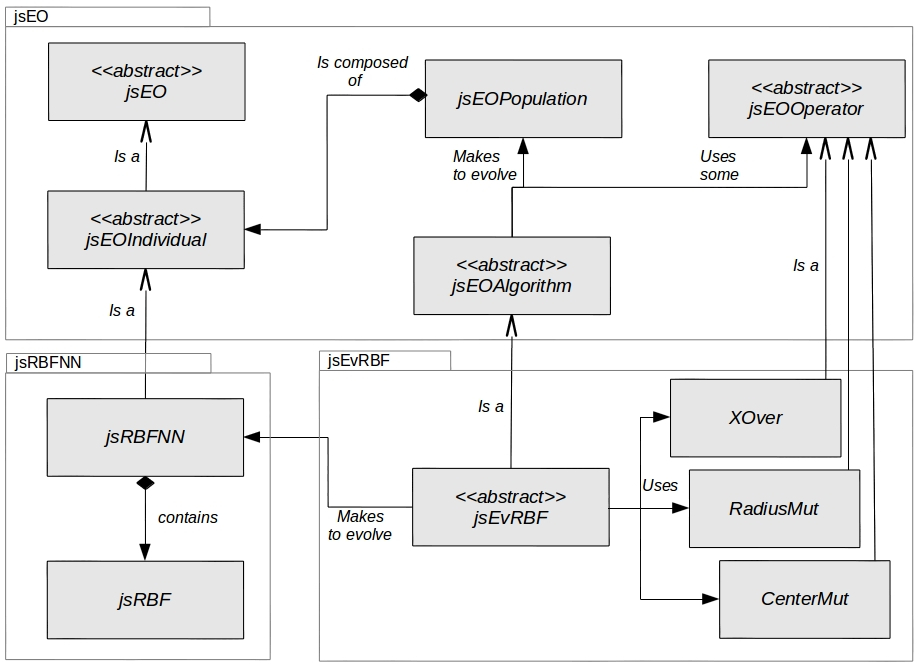
\includegraphics[width=120mm]{class-diagram.jpg}
\caption{Class diagram of the jsEvRBF algorithm, showing the way it depends on the jsEO general framework and the jsRBFNN library.}
\label{fig:class_diagram}
\end{figure}


%The individuals are RBFNN, any of them composed of a set of hidden neurons implemented as a vector of objects. Every hidden neuron stores its center and radius, and the global RBFNN stores the weights and bias. 
The fitness is computed using the inverse of the RMSE, so the greater fitness, the better the individual. 

With respect to the operators used in this algorithm:

\begin{itemize}
\item {\em XOver.} Takes two individuals as inputs and operates by randomly selecting a set of neurons from first individual and another set (probably of a different size) from the second one. After this, those sets are interchanged.
\item {\em CenterMut.} Modifies a percentage of the centers of the individual it gets as input, just setting the new center to random values in the range defined by the input dimension.
\item {\em RadiusMut.} Quite similar to the precendent, this operator modifies a percentage of the radius of the neurons belonging to the individual received, choosing a new value in the same way the {\em CenterMut} operators does.
\end{itemize}


Finally, the following set of parameters has to be established in order to run the {\em jsEvRBF} algorithm:
\begin{itemize}
\item{\em trnSamples}: Set of samples to train the nets; it will be also used to select the centers of the RBF of individuals in the initial population.
\item{\em valSamples}: Set of samples to compute fitness.
\item{\em inputDimension}: Dimension of inputs.
\item{\em numNeurons}: Number of neurons for individuals of first population.
\item{\em popSize}: Size of population
\item{\em numGenerations}: Number of generations for the evolutionary algorithm.
\item{\em tournamentSize}: Number of individuals to consider when selecting one of them to reproduce.
\item{\em replaceRate}: Rate of individuals to be replaced in every new generation.
\item{\em xOverRate}: Determines the number of individuals to which xOver operators will be applied.
\item{\em mutRate}: Determines the number of individuals to which mutator operators will be applied.
\item{\em mutPower}: Determines the number of neurons that will be changed by mutator operators, once the are being applied to a given individual.
\end{itemize}

Next section shows the exact values used for any of this parameters along the execution of the experiments.
% Specific characteristics of this implementation
% Operators
\section{Experiments and results}
\label{sec:experiments}
% The data-set
In order to test the performance of {\em jsEvRBF}, the algorithm has been evaluated with the time-series used by Sheta and de Jong \cite{Sheta2001}. It is composed of 208 weekly averaged observations representing the exchange rates between Bristish pound and US dollar from 31 December 1979 to 26 December 1983\footnote{The source of the information, thanks to the work done by Prof. Werner Antweiler from the University of British Columbia, Vancouver, Canada, is available from \url{http://pacific.commerce.ubc.ca/xr/data.html}.}. This data set has been used in a similar way than Sheta and de Jong: only half the data (randomly choosen) has been used to train and validate the nets, but the generalization error has been computed over the whole data set.

% Two kind of experiments?
Two experiments have been carried out using {\em jsEvRBF}. First one has been open to a wide community of users, so that many different devices, operating systems and web browsers have been used. 
On the other hand, the second experiment has been executed in a single computer, using a single web browser, so that we can focus in the forecasting process itself.
In any case, participating in the experiment only required to connect to an URL; no special technical knowledge was necessary to run the algorithm since it was automatically executed once the web page was loaded. 
%Figure \ref{fig:example-of-execution} shows the page users could read when accessing the specified URL.
% As can be seen, it emulated the look of a paper and need not actions to be performed by the user.

Information about clients and the results they yielded were received by a server programed also in JavaScript (using {\em node.js}) and stored in a No-SQL database managed by {\em Mongo}; the language to query the database was JavaScript too.

%
%\begin{figure}[!ht]
%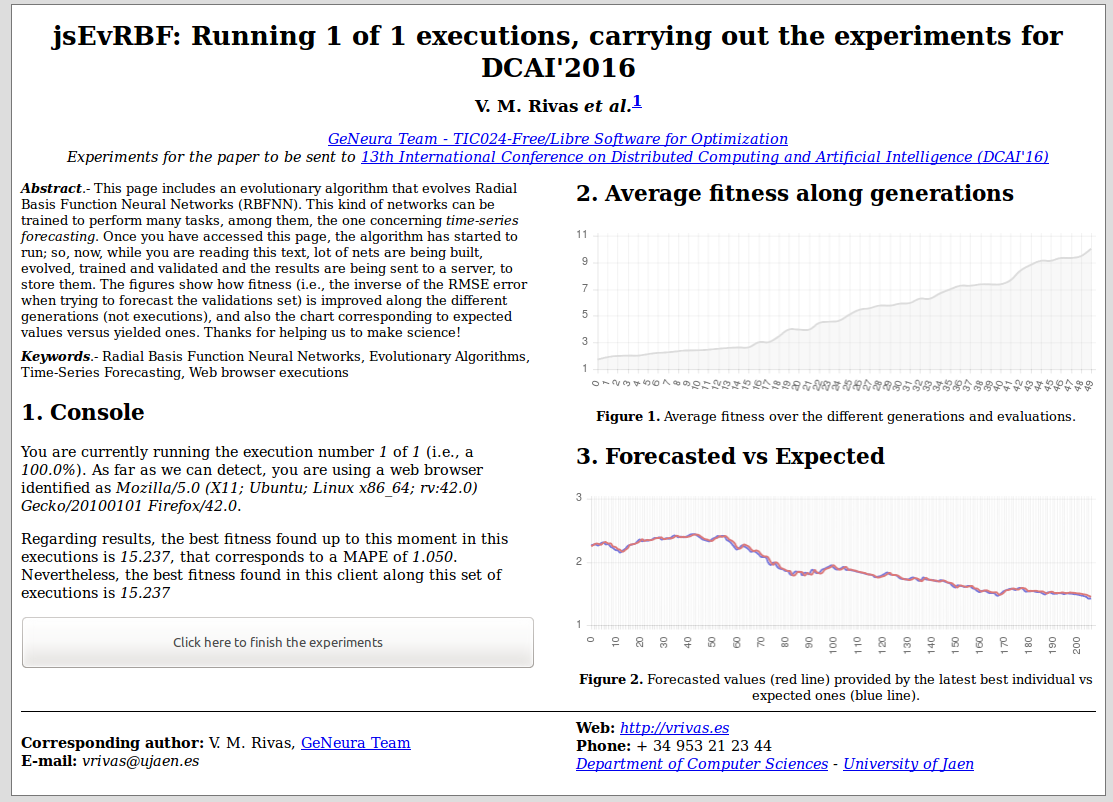
\includegraphics[width=120mm]{example-of-execution.png}
%\caption{The look of the web page in which the {\em jsEvRBF} algorithm was loaded and executed.}
%\label{fig:example-of-execution}
%\end{figure}

% First one: lot of different browsers, short executions
\subsection{First experiment: short executions, many browsers}
\label{sec:first-experiment}
The first experiment carried out was designed to test whether the kind of computation described by {\em jsEvRBF} could be effectively executed in different platforms. To do this, a "call for volunteer computation" in the form of messages published in Twitter and Facebook was done. Any of these two accounts were followed by about 500 people. %, although messages were also re-distributed by some of the original followers. The profile of Twiitter followers was mainly technical (IT professional and/or students), being more varied in the case of Facebook ones. 


Table \ref{tab:parameters-first-experiment} shows the value specified for every parameter. They differ from the ones used in previous work \cite{Rivas04} due to the lack of power of low-quality, old smartphones. An initial test showed that browsers running in that kind of devices usually blocked the execution of the algorithm; this led us to configure the experiment paying more attention to the algorithm's ability  to be executed in any device more than in its ability to perform the best forecasting.

\setlength{\tabcolsep}{10pt}
\begin{table}
\caption{Values for parameters in the first experiment. The number of samples ({\em trnSamples} and {\em valSamples}) are approximated as they were randomly chosen in every execution:  approximately $45\%$ of data were used for training, and $5\%$ for validation.}
\label{tab:parameters-first-experiment}
\begin{center}
\begin{tabular}{rr|rr}
{\bf Parameter} & {\bf Value} & 
{\bf Parameter} & {\bf Value}\\
\hline
{\em trnSamples} & $\approx 90$ &
{\em valSamples} & $\approx 15$  \\
{\em inputDimension} &   1 &
{\em numNeurons} &  7 \\
{\em popSize} &  10 &
{\em numGenerations} & 10  \\
{\em tournamentSize} &  2 &
{\em replaceRate} &   0.8 \\
{\em xOverRate} &  {\em Not used}&
{\em mutRate} &   1.0  \\
{\em mutPower} &  0.5 & {\em Executions per page load} & 15\\
\hline
\end{tabular}
\end{center}
\end{table}

This experiment was available for users from 8-Jan-2016 to 18-Jan-2016. Every time a user accessed to the URL, 15 independent executions of the algorithm were sequentially run in his/her web client. The user could easily stop these executions in any moment these executions. After every execution, results were sent to our server to store a description of the web browser, and a set of error values including MSE among others. 

The analysis of the results showed that a total of $165$ different access were made to the page during the cited period, resulting in $2304$ executions, i.e.,  $13.9$ executions in average per client. Up to 25 different versions of browser were detected, more than a half were Chrome browsers ($58.79\%$), followed by Safari ($26.06\%$) and Firefox($15.15\%$). Unfortunately, only $80\%$ of the solutions were valid, since in some executions performed by Chrome and Safari browsers (i.e., those based on AppleWebKit) a $NaN$ error appeared when training the nets.  This can be considered one of our first conclusions since, even having used standard javaScript code, there exist differences in the way browsers compile it.

With respect to forecasting, table \ref{tab:comparison-first-experiment} shows the MSE of the algorithm and compares with results from previous papers by Rivas \cite{Rivas04} and Sheta \cite{Sheta2001}. The average MSE of {\em jsEvRBF} with respect to the rest of methods is quite high ($2$ orders of magnitude). This is also due to the previously cited non-valid solutions found by AppleWebKit-based browsers: once the training fails, nets can't evolve and no better solutions than those found in initial generations are built.  As table \ref{tab:comparison-first-experiment} shows, the best solution found by the entire set of browsers is $6 \times 10^{-4}$, similar to the average error found by the original {\em EvRBF} algorithm. This is true not only for the best solution: the average MSE of the best 50 solutions is still $6 \times10^{-4}$, while the average MSE of the best 500 solutions is equal to that value for the MSE-LSE algorithm. In any case, the algorithm, as it is currently implemented, shows a lack of robustness that needs to be tackled and fixed.

%Finally, table \ref{tab:all-error-values-experiment-1} shows the rest of error-measure values yielded by {\em jsEvRBF}, in order to easier future works. 


\setlength{\tabcolsep}{10pt}
\begin{table}
\caption{First experiment: comparison of MSE yielded by the {\em jsEvRBF} algorithm and the ones cited in \cite{Rivas04}. Errors have computed over the full set of data.}
\label{tab:comparison-first-experiment}
\begin{center}
\begin{tabular}{lcc}
{\bf Method} & {\bf Average MSE} & {\bf Best MSE} \\
\hline
EvRBF & $6 \times 10^{-4} \pm 2 \times 10^{-4}$ &$4 \times 10^{-4}$ \\
MSE-GA & $9 \times 10^{-4}$ & N/A \\
MSE-LSE &  $12 \times 10^{-4}$ & N/A \\
{\em jsEvRBF} & $2 \times 10^{-2} \pm 5 \times 10^{0}$ & $6\time10^{-4}$  \\
\hline
\end{tabular}
\end{center}
\end{table}

%% Codigo para conseguir la tabla (previamente, copiar los datos en a
%var tmp="";
%var dob=false;
%a.forEach( function(e){
%tmp+=e.measure+" & $"+ parseFloat( e.values.average).toExponential(4)+" \\pm "+parseFloat(e.values.desvest).toExponential(4)+"$ "+((dob)?"\\":" & ")+"\n";
%dob=!(dob);
%})

%\setlength{\tabcolsep}{3pt}
%\begin{table}
%\caption{First experiment: complete set of error measures yielded {\em jsEvRBF} computed over the entire set of data.}
%\label{tab:all-error-values-experiment-1}
%\begin{center}
%\begin{tabular}{lc|lc}
%{\bf Error Measure} & {\bf Value} & {\bf Error measure} & {\bf Value} \\
%\hline
%
%MSE & $2.0916e-2 \pm 5.3016e+0$ &
%RMSE & $9.6086e-2 \pm 2.1416e+1$ \\
%MAE & $8.0802e-2 \pm 1.5650e+1$ &
%MdAE & $8.1066e-2 \pm 2.0277e+1$ \\
%MAPE & $4.6095e+0 \pm 5.6024e+4$ &
%MdAPE & $4.3373e+0 \pm 6.1799e+4$ \\
%RMSPE & $5.6733e+0 \pm 8.3952e+4$ &
%RMdSPE & $4.3373e+0 \pm 6.1799e+4$ \\
%sMAPE & $4.3511e+0 \pm 4.0497e+4$ &
%sMdAPE & $4.1231e+0 \pm 4.9165e+4$ \\
%MASE & $4.4171e+0 \pm 4.6814e+4$ &
%RMSSE & $5.2422e+0 \pm 6.3764e+4$ \\
%MdASE & $4.4267e+0 \pm 6.0254e+4$ \\
%
%\hline
%\end{tabular}
%\end{center}
%\end{table}



% Second one: only one browser, complete executions
\subsection{Second experiment: long executions, one browser}
\label{sec:second-experiment}

Once detected the error introduced by AppleWebKit-based browsers, a second experiment was carried out in a more controlled environment, and with a configuration similar to the original experiments in \cite{Rivas04}. These new executions were run using a Firefox 44 browser, and configured as showed in table \ref{tab:parameters-second-experiment}.

\setlength{\tabcolsep}{10pt}
\begin{table}
\caption{Configuration of parameters for the second experiment. As in the first one, the number of samples ({\em trnSamples} and {\em valSamples}) is still approximated since they were randomly chosen in every execution. Values that differ from experiment 1 have been highlighted in {\bf bold}}
\label{tab:parameters-second-experiment}
\begin{center}
\begin{tabular}{rr|rr}
{\bf Parameter} & {\bf Value} & 
{\bf Parameter} & {\bf Value}\\
\hline
{\em trnSamples} & $\approx 90$ &
{\em valSamples} & $\approx 15$  \\
{\em inputDimension} &   1 &
{\em numNeurons} &  {\bf 10} \\
{\em popSize} &  {\bf 15} &
{\em numGenerations} & 10  \\
{\em tournamentSize} &  {\bf 3} &
{\em replaceRate} &   {\bf 0.2} \\
{\em xOverRate} &  {\bf 0.2}&
{\em mutRate} &   {\bf 0.8}  \\
{\em mutPower} &  0.5 & 
{\em Executions per page load} &  {\bf 1} \\
\hline
\end{tabular}
\end{center}
\end{table}

The results for this second experiments, averaged over 10 executions of the algorithm, were clearly better than those yielded in first one, as can be seen in table \ref{tab:comparison-second-experiment}. Although the original {\em EvRBF} algorithm still yields the best result ($6 \times 10^{-4} \pm 2 \times 10^{-4}$), {\em jsEvRBF} can be compared in this occasion with it ($8 \times 10^{-4} \pm 2 \times 10^{-7}$), and is lower than MSE-GA ($9 \times 10^{-4}$) and MSE-LSE ($12 \times 10^{-4}$). Further study must be done to determine the causes that makes the new algorithm being not so accurate as the original one, but probably the absence of some of the operators not yet programed could be the reason.

\setlength{\tabcolsep}{10pt}
\begin{table}
\caption{Second experiment: comparison of MSE yielded by the {\em jsEvRBF} algorithm and the ones cited in \cite{Rivas04}. Errors have computed over the full set of data, having executing the algorithm 10 times.}
\label{tab:comparison-second-experiment}
\begin{center}
\begin{tabular}{lcc}
{\bf Method} & {\bf Average MSE} & {\bf Best MSE} \\
\hline
EvRBF & $6 \times 10^{-4} \pm 2 \times 10^{-4}$ &$4 \times 10^{-4} \pm 2 \times 10^{-4}$ \\
{\em jsEvRBF} & $8 \times 10^{-4} \pm 2 \times 10^{-7}$ & $6\times10^{-4}$  \\
MSE-GA & $9 \times 10^{-4}$ & N/A \\
MSE-LSE &  $12 \times 10^{-4}$ & N/A \\
\hline
\end{tabular}
\end{center}
\end{table}

%Finally, and as we did before, table \ref{tab:all-error-values-experiment-2} summarizes the values computed for this experiment with regard to the complete set of error measures.
%
%\setlength{\tabcolsep}{3pt}
%\begin{table}
%\caption{Second experiment: complete set of error measures yielded {\em jsEvRBF} computed over the entire set of data.}
%\label{tab:all-error-values-experiment-2}
%\begin{center}
%\begin{tabular}{lc|lc}
%{\bf Error Measure} & {\bf Value} & {\bf Error measure} & {\bf Value} \\
%\hline
%
%MSE & $7.5601e-4 \pm 1.6728e-7$  & 
%RMSE & $2.7398e-2 \pm 5.3461e-5$ \\
%MAE & $2.1099e-2 \pm 3.4528e-5$  & 
%MdAE & $1.6385e-2 \pm 4.0988e-5$ \\
%MAPE & $1.1091e+0 \pm 1.0119e-1$  & 
%MdAPE & $8.7471e-1 \pm 1.2897e-1$ \\
%RMSPE & $1.4293e+0 \pm 1.5105e-1$  & 
%RMdSPE & $8.7471e-1 \pm 1.2897e-1$ \\
%sMAPE & $1.1065e+0 \pm 9.8722e-2$  & 
%sMdAPE & $8.7381e-1 \pm 1.2609e-1$ \\
%MASE & $1.1515e+0 \pm 1.0601e-1$  & 
%RMSSE & $1.4940e+0 \pm 1.6138e-1$ \\
%MdASE & $8.9537e-1 \pm 1.2759e-1$  \\
%\hline
%\end{tabular}
%\end{center}
%\end{table}


\section{Conclusions}
\label{sec:conclusions}
In this paper, web-browsers have been proved to be a good alternative to achieve
distributing computation, minimizing the effort needed to ensure
cross-platform compatibility as well as easiness of use. To show it, we have introduced the {\em jsEvRBF} algorithm;
written in JavaScript, this algorithm can be executed in web-browsers
when users access to a specified URL. The web page downloaded by the
web-browser contains the code of this evolutionary algorithm, able to
build, train and evolve RBFNN used to perform time-series forecasting
over a set of data related to currency exchange. % which is
                                % interesting because... -JJ

The experiments carried so far show that the approach is valid,
although some research must still be done in order to determine the
reasons that make AppleWebKit-based browsers (mainly Chrome and
Safari) not work properly, yielding poor results with respect to forecasting error.


% never negative statements: say you are going to do it the future
% - JJ
Future work includes the use of the
algorithm in an {\em island model}  framework in which good
individuals be distributed to the clients running the algorithm, since {\em jsEO}, the underlying
library supporting {\em jsEvRBF}, has been implemented with this
feature. 



\section*{Acknowledgements}
 This work has been supported in part by projects: TIN2011-28627-C04-02 awarded by the Spanish Ministry of Economy and Competitivity, SPIP2014-01437 (PETRA project, funded by Direcci�n General de Tr�fico), 
PRY142/14 (Este proyecto con num. de referencia: PRY142/14 ha sido financiado �ntegramente por la Fundaci\'{o}n P\'{u}blica Andaluza Centro de Estudios Andaluces en la IX Convocatoria de Proyectos de Investigaci\'{o}n)\footnote{The description in Spanish is mandatory.}, and PYR-2014-17 GENIL project, awarded by CEI-BIOTIC Granada.

%
% ---- Bibliography ----
%
\begin{thebibliography}{}
%
%\bibitem[1980]{2clar:eke}
%Clarke, F., Ekeland, I.:
%Nonlinear oscillations and
%boundary-value problems for Hamiltonian systems.
%Arch. Rat. Mech. Anal. 78, 315--333 (1982)

\bibitem[2]{Broomhead88}
Broomhead, D.S., Lowe D.: Multivariable functional interpolation and adaptive networks. Complex Systems, 2, 321--355 (1988)

\bibitem[3]{Champeon08}
Champeon S.: JavaScript: How Did We Get Here?. MySQL Conference and Expo, Santa Clara, CA (2008)

\bibitem[4]{Eich2010}
Brendan E.: A Brief History of JavaScript. http://bit.ly/1lKkI0M (2010)

\bibitem[5]{Flanagan06}
Flanagan D.: JavaScript: The Definitive Guide. O'Reilly Media, Inc. (2006)

\bibitem[6]{Keogh03}
Keogh, E.: On the Need for Time Series Data Mining Benchmarks: A Survey and Empirical. Data Mining and Knowledge Discovery, 7(4), 349--371 (2003).

\bibitem[7]{Rauschmayer04}
Rauschmayer A.: Speaking JavaScript. An In-Depth Guide for Programmers. O'Reilly Media, ISBN: 978-1-4493-6503-5 (2004)

\bibitem[8]{Rivas04}
Rivas, V.M., Merelo, J.J., Castillo, P.A., Arenas, M.G., Castellanos, J.G.: Evolving RBF neural networks for time-series forecasting with EvRBF. Information Sciences, 165(3-4), 207--220 (2004)

\bibitem[9]{RivasEvoStar2014}
Rivas, V.M.,  Merelo, J.J., Romero,  G., Garcia-Arenas, M., Mora, A.: An Object-Oriented Library in JavaScript to Build Modular and Flexible Cross-Platform Evolutionary Algorithms, in Applications of Evolutionary Computation - 17th European Conference, EvoApplications 2014, Granada, Spain, April 23-25, (2014)

\bibitem[10]{Whitehead}
Whitehead, B., Choate, T.: Cooperative-competitive genetic evolution of Radial Basis Function centers and widths for time series predictioN. IEEE Trans. on Neural Networks, 7(4), 869--880 (1996).

\bibitem[11]{Sheta2001} 
Sheta, A.F., de Jong, K.: Time-series forecasting using GA-tuned radial basis functions,Information Sciences 133 (3?4)  221--228, April.(2001)

\end{thebibliography}
% Don't like this at all... using .bib much better.
%\addtocmark[2]{Author Index} % additional numbered TOC entry
%\renewcommand{\indexname}{Author Index}
%\printindex
%\clearpage
%\addtocmark[2]{Subject Index} % additional numbered TOC entry
%\markboth{Subject Index}{Subject Index}
%\renewcommand{\indexname}{Subject Index}
%\input{subjidx.ind}
\end{document}
